\documentclass[../main.tex]{subfiles}

\graphicspath{{\subfix{../imgs/}}}

\begin{document}

\section{Litterature}
\begin{frame}[c]
    \frametitle{Litterature}

    \begin{block}{Papers}
        \begin{itemize}
            \item PanNuke Dataset Extension, Insights and Baselines (2020).
            \item A Novel Dataset for Nuclei Segmentation in Melanoma Histopathology (2024).
        \end{itemize}
    \end{block}
\end{frame}

\begin{frame}[t]
    \frametitle{Litterature}
    \textbf{A Novel Dataset for Nuclei Segmentation in Melanoma Histopathology (2024)}

    \vspace{20pt}
    Argues the use of models trained exclusively on melanoma data, as opposed to the PanNuke dataset. Sees good results with Mask R-CNN and HoverNet.

    \begin{figure}[h]
        \centering
        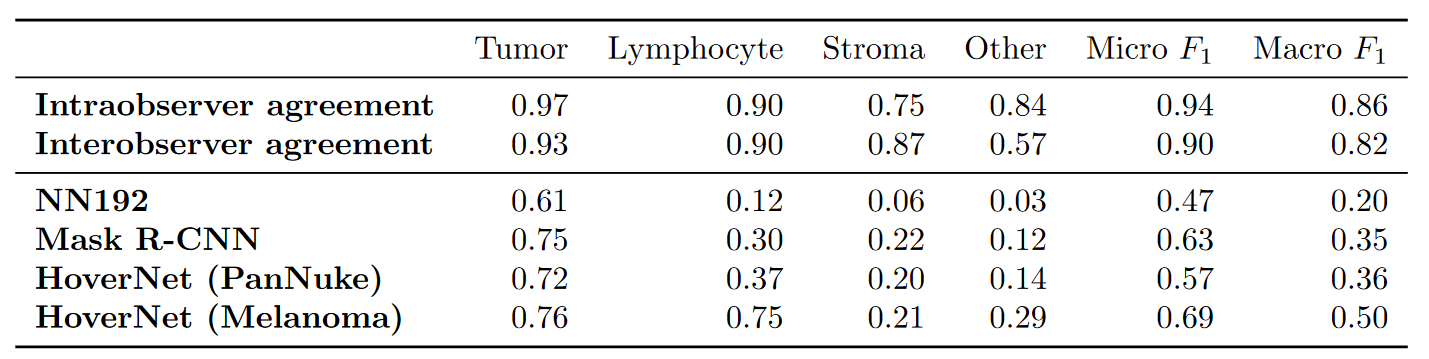
\includegraphics[width=1\textwidth]{paper_table_1.png}
        \caption{$F_1$ scores for inter/intraobserver and different models.}
    \end{figure}
\end{frame}

\end{document}